\documentclass[tikz,border=10pt]{standalone}
\begin{document}
  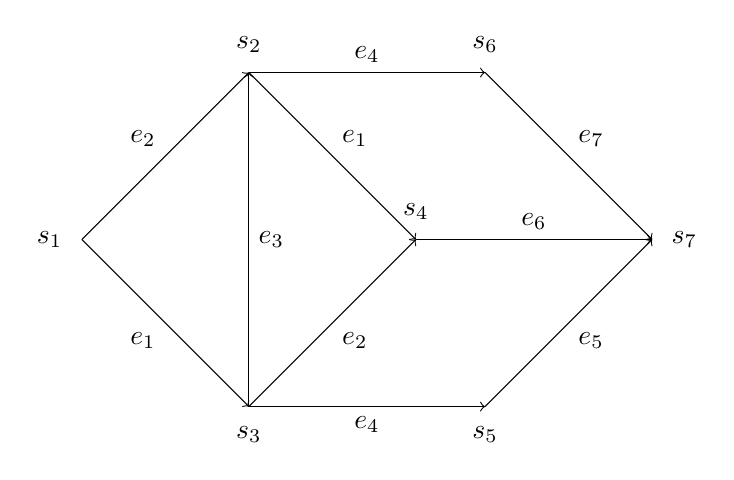
\begin{tikzpicture}[node distance=3cm, align=center]
    \title{A transition system}

    \node(q1) [label=left:{$s_{1}$}]                        {};
    \node(q2) [above right of=q1, label=above:{$s_{2}$}]    {};
    \node(q3) [below right of=q1, label=below:{$s_{3}$}]    {};
    \node(q4) [below right of=q2, label=above:{$s_{4}$}]    {};
    \node(q5) [right of=q3, label=below:{$s_{5}$}]          {};
    \node(q6) [right of=q2, label=above:{$s_{6}$}]          {};
    \node(q7) [right of=q4, label=right:{$s_{7}$}]          {};
    
    \draw [->][draw=black] (q1.center) to node [above left] {$e_{2}$} (q2.center);
    \draw [->][draw=black] (q1.center) to node [below left] {$e_{1}$} (q3.center);
    \draw [->][draw=black] (q2.center) to node [above right] {$e_{1}$} (q4.center);
    \draw [->][draw=black] (q3.center) to node [right] {$e_{3}$} (q2.center);
    \draw [->][draw=black] (q3.center) to node [below] {$e_{4}$} (q5.center);
    \draw [->][draw=black] (q2.center) to node [above] {$e_{4}$} (q6.center);
    \draw [->][draw=black] (q3.center) to node [below right] {$e_{2}$} (q4.center);
    \draw [->][draw=black] (q4.center) to node [above] {$e_{6}$} (q7.center);  
    \draw [->][draw=black] (q5.center) to node [below right] {$e_{5}$} (q7.center);
    \draw [->][draw=black] (q6.center) to node [above right] {$e_{7}$} (q7.center);

  \end{tikzpicture}
\end{document}